\chapter{Concept}
\label{cha:methoden}

This chapter presents the current state of mobile navigation with ROS and its limitations. This chapter aims to identify the critical areas in which standard mobile robots running ROS lack robustness and autonomy during autonomous mobile navigation. According to these critical areas, requirements are derived and prioritized with a risk analysis. This chapter proposes how behavior planning can improve the current default systems to meet the respective requirements. 

\section{Current State}
\label{sec:Current State}

\subsection{ROS}
The Robot Operating System (ROS) is an open-source middleware for creating robot applications. It is not an operating system (OS) since it needs an underlying OS, most commonly Linux, to work. ROS can handle the communication between different programs (called nodes) with standardized interfaces and network protocols. Nodes can communicate via topics, services, and actions, which differ in their application domain (compare table \ref{tab:ros_interfaces}). 

\begin{table}[ht]
	\centering
	\caption{ROS Communication Options}
	\label{tab:ros_interfaces}
	\renewcommand{\arraystretch}{1.5}
	\resizebox{0.95\textwidth}{!}{%
		\begin{tabular}{ | m{0.09\textwidth} | m{0.37\textwidth}| m{0.45\textwidth} | m{0.139\textwidth}|} 
			\hline
			\textbf{Name} & \textbf{Communication Pattern} & \textbf{Area of Use} & \textbf{Cardinality} \\ 
			\hline
			Topics & Publisher / Subscriber & Continuous stream of data (e.g. sensor data) & n:m \\ 
			\hline
			Services & Request / Response & Get specific data only once & One service, many clients \\ 
			\hline
			Actions & Request / Response and Publish / Subscribe & Trigger executing of asynchronous goal-driven processes and receive updates & One action, many clients \\
			\hline
		\end{tabular}
	}
\end{table}

This design choice makes robotic applications built with ROS highly reusable and interchangeable, allowing developers to integrate foreign libraries more easily into their applications. Due to the availability of many high-quality open-source libraries for many different use cases, ROS has become the leading methodology for creating robotic applications in the research environment \cite{quigley2009}. 

With ROS2, the framework received fundamental changes and updates to its architecture and design to gain more acceptance and increased usage in the industry. These changes allow for real-time safety, simpler certification, and security when building industrial applications and products using ROS2 \cite{ros2022}. 

\subsection{Turtlebot3}
\label{subsec:Turtlebot3}

The Turtlebot3 is a standard mobile research platform with an available ROS interface to control the robot. The robot is well-integrated into the ROS ecosystem and is established in the literature as a system to develop and integrate new methods. The robot has two motors with attached wheel encoders to drive and steer, classifying it as a differential drive robot. A third omnidirectional wheel stabilizes the robot. 

The manufacturer provides an open-source model for simulating the robot in physics-based simulators like Gazebo, as depicted in figure \ref{fig:turtlebot}, which enables faster development and testing of the created robotic applications.

\begin{figure}[ht]
	\centering
	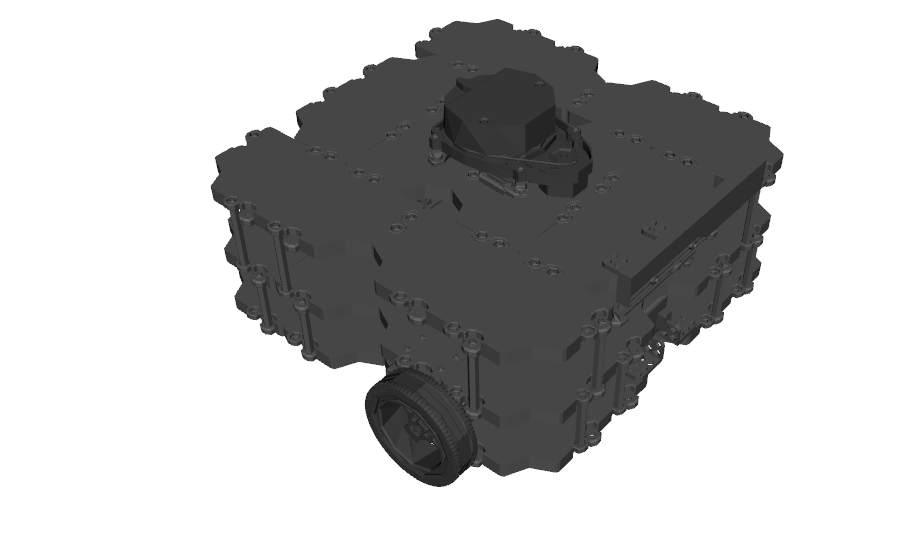
\includegraphics[width=0.3\textwidth]{images/turtlebot_sim.png}
	\caption{Turtlebot3 model in Gazebo simulator}
	\label{fig:turtlebot}
\end{figure}

The equipped sensors and easy simulation capabilities make the robot well-suited for using the Navigation2 stack and further development for behavior planning. The robot specifications are specified in table \ref{tab:turtlebot_spec} (p.\pageref{tab:turtlebot_spec}). The turtlebot will be used to analyze the current state of mobile navigation. Furthermore, the simulated turtlebot will be the platform where the behavior planning will be implemented and tested.

\begin{table}[ht]
	\centering
	\caption{Turtlebot3 Specifications}
	\label{tab:turtlebot_spec}
	\renewcommand{\arraystretch}{1.5}
	\resizebox{0.8\textwidth}{!}{%
		\begin{tabular} {| l | l |} 
			%{| m{0.3\textwidth} | m{0.3\textwidth} |} 
			\hline
			\textbf{Specification} & \textbf{Value} \\ 
			\hline
			Maximum translational velocity & 0.26 m/s \\ 
			\hline
			Maximum rotational velocity & 1.82 rad/s (104.27 deg/s) \\
			%	 	\hline
			%	 	Maximum payload & 30kg \\
			\hline
			Size (L x W x H) & 281mm x 306mm x 141mm \\
			\hline
			Singe Board Computer & Raspberry Pi (3 or 4) \\
			\hline
			Laser Distance Sensor (Lidar) & 360 Degree Laser Distance Sensor LDS-01 \\
			\hline
			Inertial Measurement Unit (IMU) & Gyroscope 3 Axis, Accelerometer 3 Axis \\
			\hline
			Actuators & XM430-W210 \\
			\hline
		\end{tabular}
	}
\end{table}

\subsection{Navigation2}
\label{subsec:nav2}

The ROS Navigation2 Stack (Nav2) combines different packages that allow mobile robots to navigate from point A to point B. Navigation2 is the de-facto standard for mobile navigation with a wide range of supported robots. Supported robot types are holonomic, differential-drive, legged, and ackerman (car-like). For the mobile robot to make use of the Nav2 stack, it has to be set up in a certain way to be able to generate plans and execute commands in the right way. The Nav2 setup requires the mobile robot to possess a laser scan or point cloud sensor, an odometry source (such as an Inertial Measurement Unit (IMU) or wheel encoders), a map with information about free and occupied spaces (Occupancy Grid Map (OGM)), and a set of transformations for planning and navigation (see figure \ref{fig:nav_architecture}). 

\begin{figure}[ht]
	\centering
	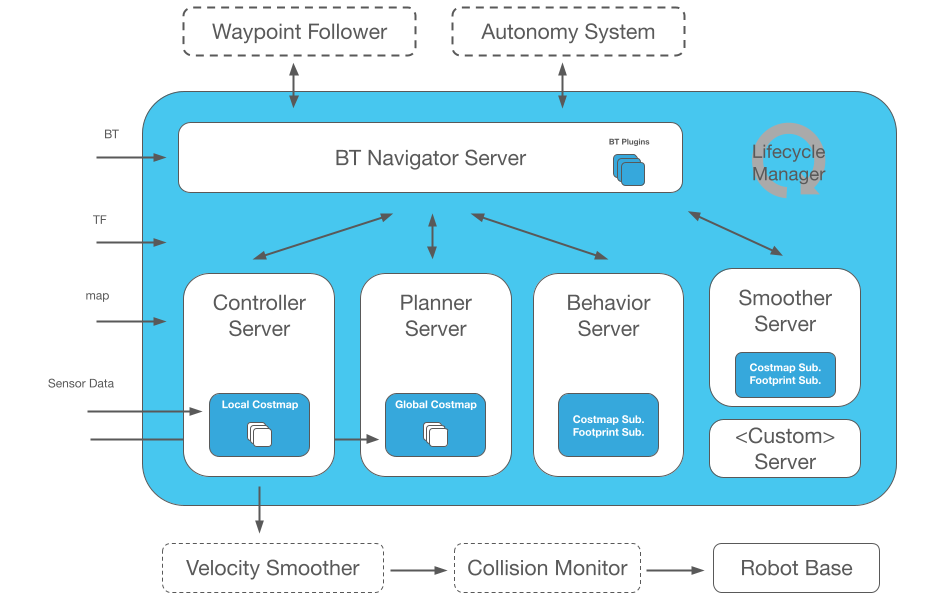
\includegraphics[width=0.9\textwidth]{images/nav2_architecture.png}
	\caption{Navigation2 Architecture \cite{macenski2020}}
	\label{fig:nav_architecture}
\end{figure}

The stack contains tools that save and load occupancy maps, localize the robot, plan paths, execute the path, provide cost maps, build behaviors, and execute recoveries \cite{macenski2020}. These packages are often integrating a Simultaneous Localization and Mapping (SLAM) method to build or enlarge maps. Path planning and execution capabilities, which correspond to the global and local planner described in section \ref{sec:Autonomous Driving Navigation Architectures}, are further supported by ready-to-use planning plugins that use A* and Dijkstra algorithms for global path planning and a dynamic window approach for path execution (local planning). The system sequencing is done in a hierarchical structure as a central behavior tree calls asynchronous actions from the respective planners after another, as seen in figure \ref{fig:nav_architecture} on page \pageref{fig:nav_architecture}. 

\begin{figure}[ht]
	\centering
	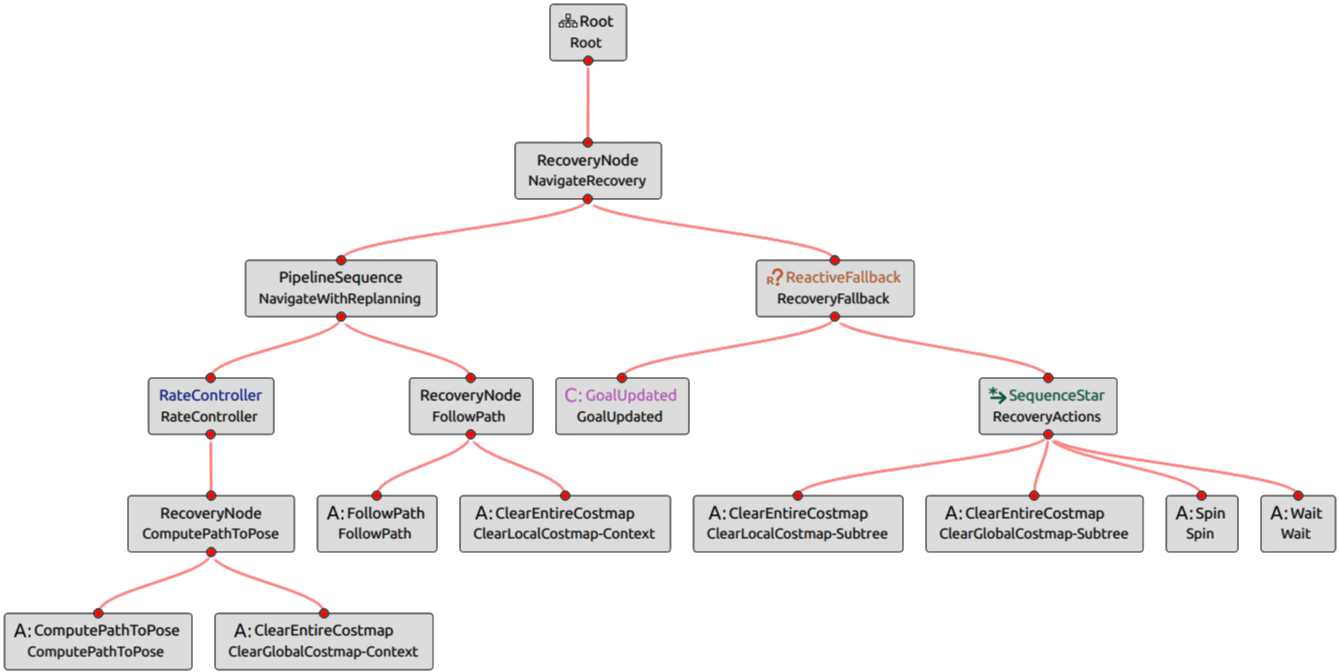
\includegraphics[width=0.9\textwidth]{images/nav_bt-modified.png}
	\caption{Navigation2 Behavior Tree}
	\label{fig:bt_nav}
\end{figure}

The behavior tree depicted in figure \ref{fig:bt_nav} is the default Nav2 behavior and has a set of recovery behaviors already implemented (spin, wait, back up, clear map). These behaviors are executed if the robot can not progress towards the set goal. Nav2 uses a node lifecycle management system to start, activate, deactivate, and shut down nodes in a controlled way. The lifecycle approach allows the system to monitor the system nodes' startups, executions, and failures.

With this quantity of functions and hierarchical architecture, the ROS Navigation2 stack is an excellent basis for achieving high levels of robot autonomy. The software can be modified and expanded with plugins to fit the users' needs. When comparing the functionalities of the software stack to the proposed autonomous system architecture in figure 	\ref{fig:autonomous_driving_architecture}, the functionalities that Navigation2 is missing are a system-wide supervision layer and a more deliberative approach to behavior planning (as mentioned in section \ref{sec:Behavior Types}).

The absence of these components leads to a limited set of circumstances in which the robot can perform navigation reliably. One of the core problems behavior-based robots face is generating a dependable environment representation. An accurate representation is the basis for the last steps in the planning part of the \textit{"Sense - Think - Act"} cycle. Unforeseen events can severely limit the reliability of the environment representation without the robot detecting the unreliability. 

Examples of such events currently not handled appropriately are slipping wheels, orientation changes by external influences, or undetected, more specifically, undetectable obstacles. These events can lead to erratic movement of the robot, as reactive behaviors and more deliberative behaviors compete for authority over the robot's movement. By design, to allow more intelligent robot behaviors, the deliberative behavior can override commands from reactive behaviors. However, the deliberative behavior's planning is based upon a false representation of reality, leading to incorrect commands. 

The unsafe planning triggers reactive-type behaviors again to counteract the commands from the deliberative behavior. In a more severe scenario, the reactive behaviors may not get activated, and the robot continues to drive despite the incorrect interpretation of the surroundings. This highly unsafe behavior requires a human operator to step in and restore the robot manually to full functionality. 
%\textit{Add a closing statement about that suitability of the Nav stack for achieving autonomy}

\section{Requirements}
\label{sec:Requirements}

The software requirements that improve the robot's behavior are derived from the current limitations of the standard ROS and Navigation2 setup for mobile robots described in the previous section. The non-functional requirements are listed separately in table \ref{tab:nonfn_req}. The functional requirements and their acceptance criteria are listed in table \ref{tab:fn_req} on page \pageref{tab:fn_req}. Figure \ref{fig:use_case} on page \pageref{fig:use_case} depicts a Use-Case diagram with the functions needed to improve the system's autonomy and better contextualize the system's requirements.

\begin{table}[ht]
	\centering
	\caption{Non-Functional Requirements}
	\label{tab:nonfn_req}
	\renewcommand{\arraystretch}{1.5}
	\resizebox{0.9\textwidth}{!}{%
		\begin{tabular}{ | m{0.11\textwidth} | m{0.14\textwidth}| m{0.1\textwidth} | m{0.7\textwidth} |} 
			\hline
			\textbf{Nr.} & \textbf{Name} & \textbf{Priority} & \textbf{Description} \\ 
			\hline
			non$\_$freq1 & Single Point of Failure & High & The system does not have a single point of failure	When parts of the system fail, the system maintains operability to a degree. \\ 
			\hline
			non$\_$freq2 & Performance & High & The system's control loop guarantees fast reactions. The average frequency with which the system operates is higher than 100Hz (10ms). \\ 
			\hline
			non$\_$freq3 & Determinism & High & The outcome for a given set of inputs must be deterministic, meaning that the behavior is always executed similarly. \\
			\hline
			non$\_$freq4 & Deliberate & High & The robot can execute deliberative behaviors, meaning that behaviors new implemented behaviors go beyond reacting to sensor input and have a planning aspect. \\
			\hline
		\end{tabular}
	}
\end{table}

\begin{table}[ht]
	\centering
	\caption{Functional Requirements}
	\label{tab:fn_req}
	\renewcommand{\arraystretch}{1.5}
	\resizebox{0.95\textwidth}{!}{%
		\begin{tabular}{| m{0.08\textwidth} | m{0.15\textwidth}| m{0.09\textwidth} | m{0.60\textwidth}|} 
			\hline
			\textbf{Nr.} & \textbf{Name} & \textbf{Priority} & \textbf{Description/Acceptance Criteria} \\ 
			\hline
			fn$\_$req1 & Sensor Failure & High & The system detects sensor failure. Ensure that the system can restart sensors and decrease the speed during the time the sensor delivers limited information. \\ 
			\hline
			fn$\_$req2 & Emergency Detection & High & The system detects emergency. Ensure that the system can detect when the continuation on the calculated path is no longer safe (sensor failures, blockage). \\
			\hline
			fn$\_$req3 & Emergency Stop & High & The system can initiate emergency stops. Ensure that the system can override all commands and stop in case an emergency is detected. \\
			\hline 	
			fn$\_$req4 & Override Navigation2 & High & The system can override navigation2. Ensure that the system's commands can always override the commands coming from navigation2. \\
			\hline
			fn$\_$req5 & Maintain operability & High & The robot executes commands as long as it is safe. Ensure that the robot keeps driving if it is safe even when system functions are not working correctly. \\
			\hline
			fn$\_$req6 & Recovery & High & The system can recover from crashes. Ensure that the system can successfully reach goals despite previous crashes.\\ 
			\hline 
			fn$\_$req7 & Control Path Planning & Medium & The system controls and rates the quality of the planned paths. \\
			\hline	
			fn$\_$req8 & Reset Goals & Medium & The system can reset and override goals set by the user so that the goal is reachable by planners. \\
			\hline
			fn$\_$req9 & Robot Range & Medium & Ensure that the robot will not run out of battery during navigation to a goal. \\	
			\hline
		\end{tabular}
	}
\end{table}

The prioritization is based on the severity of the consequences for the system. The functional requirements one to six focus on safety and robustness of the robot and are therefore prioritized high. Functional requirements seven to nine focus on extending the autonomy of the robot, but a failure in these requirements do not pose as high of a risk the other requirements.

\begin{figure}[ht]
	\centering
	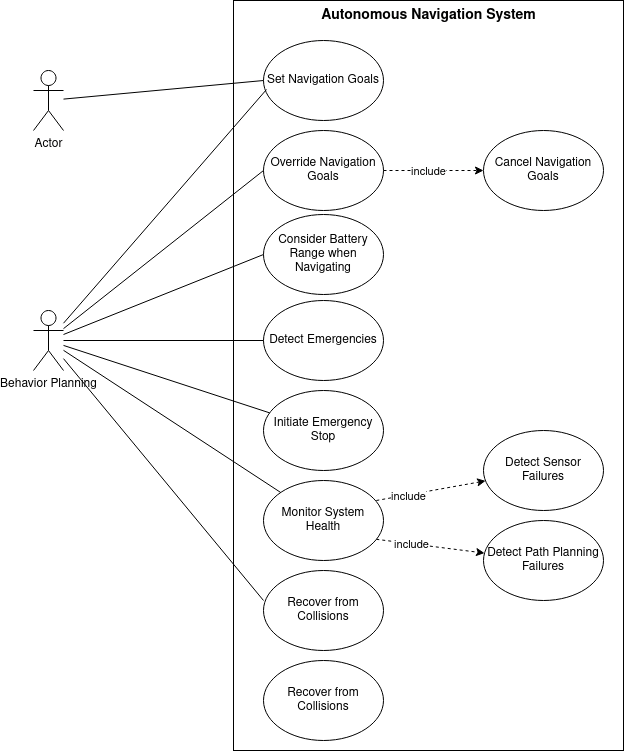
\includegraphics[width=0.7\textwidth]{images/use_case.png}
	\caption{Use Case Diagram}
	\label{fig:use_case}
\end{figure}


\section{System Solution}
\label{sec:System Solution}

For a Turtlebot3 running Nav2 to appropriately deal with the listed requirements, the system needs to be extended with new external modules. To eliminate a single point of failure for the system, one needs to create an independent second system outside the existing one. This aims to create a robust fallback behavior that does not rely on Nav2 to move. Also, an external system can more reliably monitor other systems when its execution is detached from the performance and execution of other systems.

A suitable name for the second system is the "autonomy layer", as its goal is to increase the robustness and autonomy of the whole system. The autonomy layer has to provide a comprehensive system supervisor that monitors all components' health (sensors, navigation, robot controller). The constant execution monitoring equips the system with the ability to deal with the event of node failures and component malfunctions.

Another required addition to the autonomy layer is a data storage of relevant system information and data. The stored data includes sensor data and generated maps, cost maps, positions, and speed commands. Using past data points allows behaviors to become more deliberative in their approach and opens up many possibilities for intelligent behaviors like movement predictions of obstacles. 

A third component to the autonomy layer is a behavior planner largely independent of Nav2 execution and planning. This behavior planner must be capable of overriding the Nav2 behaviors if needed. The component processes information from the execution checker, Nav2, and past and present sensor data to decide if and how to override the default behaviors. Based on this information, the behavior planner can make a deliberative, strategic decision to increase robustness and autonomy, thus decreasing reliance on human supervision.

Additionally, a component to switch intelligently between speed commands from Nav2 and the autonomy layer is needed. This component could be realized as a decision gate that receives speed commands from Nav2 and the new behavior planning component and can forward, block or modify commands sent to the controller. This modification aspect allows high-quality local planning capabilities but enables more deliberative behaviors to happen upon this planning. A simplified system block diagram is depicted in figure \ref{fig:block_diagram}. The proposed additional components discussed in this chapter are colored in blue. Existing components, discussed in section \ref{sec:Current State}, are colored in gray. 

\begin{figure}[ht]
	\centering 
	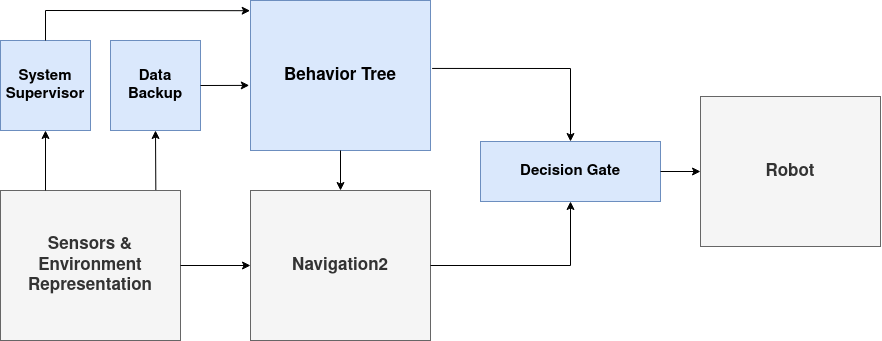
\includegraphics[width=0.9\textwidth]{images/block_diagram.png}
	\caption{System Block Diagram}
	\label{fig:block_diagram}
\end{figure}


\section{Software and Simulation}

A comparison and assessment of the behavior planning approaches were made in section \ref{sec:Behavior Planning Approaches}. The decision on which approach to use was made in favor of the behavior tree method. The main reason for this decision is the increased flexibility when creating and expanding the behavior planning compared to FSMs. Also, behavior trees allow complete determinism and introspection during execution which is why the POMPD approach is unsuitable as the primary behavior planning approach for the specified requirements. 

\subsection{Behaviortree.CPP}

The Navigation2 stack uses a behavior tree to coordinate the planning layer. The behavior tree that is used is an expansion of the Behaviortree.CPP (BT.CPP) library. This library offers a way to create, execute, monitor, and edit behavior trees. 

Additionally to the types of control nodes mentioned in section \ref{subsec:Behavior Trees}, the library adds the concept of reactivity into the catalog of control nodes. Reactive sequences and reactive fallbacks differ from normal ones in handling nodes that return the state "Running". Instead of ticking the node again, the whole sequence restarts, which is very useful for continuously checking a condition and executing an asynchronous action node that gets halted when a condition is not met anymore (see table \ref{tab:control_nodes_bt}). 

\begin{table}[ht]
	\centering
	\caption{Control Nodes in BT.CPP}
	\label{tab:control_nodes_bt}
	\renewcommand{\arraystretch}{1.5}
	\resizebox{0.8\textwidth}{!}{%
		\begin{tabular}{ | l | l | l |} 
			%			{ | m{0.2\textwidth} | m{0.25\textwidth}| m{0.25\textwidth} | m{0.2\textwidth} |} 
			\hline
			\textbf{Name }& \textbf{Child returns Failure} & \textbf{Child Returns Running} \\ 
			\hline
			Sequence & Restart & Tick Again\\ 
			\hline
			Reactive Sequence & Restart & Restart \\ 
			\hline
			Sequence Star & Tick again & Tick again \\
			\hline
			Fallback & Tick next & Tick again\\
			\hline 	
			Reactive Fallback & Tick next & Restart \\
			\hline
		\end{tabular}
	}
\end{table}

Also, the library includes another class of Control Flow Nodes, called Decorator Nodes, which allow more control over the child node and its output. An essential distinction to other Control Flow Nodes is that Decorator Nodes can only have one child node compared to multiple children for sequence and fallback nodes. A comprehensive list of the available Decorators and descriptions is presented in table \ref{tab:decorators_bt}.


\begin{table}[ht]
	\centering
	\caption{Decorator Nodes in BT.CPP}
	\label{tab:decorators_bt}
	\renewcommand{\arraystretch}{1.5}
	\resizebox{0.95\textwidth}{!}{%
		\begin{tabular}{ | m{0.15\textwidth} | m{0.4\textwidth}| m{0.4\textwidth} | m{0.2\textwidth} |} 
			\hline
			\textbf{Name} & \textbf{Succeeds} & \textbf{Fails} & \textbf{Running} \\ 
			\hline
			Inverter Node & If the child returns false & If child return success & If the child returns running \\ 
			\hline
			ForceSuccess Node & Always & Never & If child returns running \\ 
			\hline
			ForceFailure Node & Never & Always & If child returns running\\
			\hline
			Repeat Node & Ticks child as long as it returns success. Number of repeats can be defined & If the child returns failure & If the child returns running \\
			\hline 	
			Retry Node & If the child returns success & Ticks child as long as it returns failure. Number of ticks can be defined & If the child returns running \\
			\hline
		\end{tabular}
	}
\end{table}

To allow the tree nodes to communicate, the library provides the developer with two possibilities. Either node can use the blackboard, a dictionary (key/value) that all tree nodes can read and write. Alternatively, two nodes can be connected through ports which allows direct communication between two nodes via a key/value.

\subsection{Groot}

Groot is a program to create, edit, monitor, and debug behavior trees with a graphical user interface. The software allows the creation of behavior trees in XML files, which can be directly loaded into and used by the BT.CPP library. Groot can monitor the live execution of behavior trees and allows the introspection of how the tree reacts to different scenarios. Figure \ref{fig:groot} shows a small segment of an active behavior tree.

\begin{figure}[ht]
	\centering 
	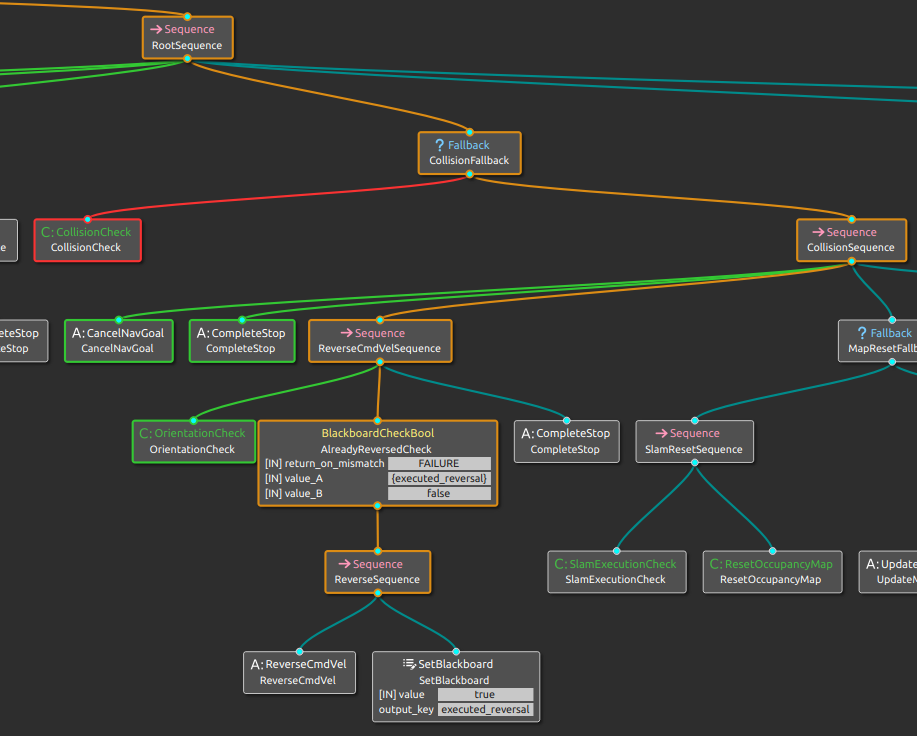
\includegraphics[width=0.9\textwidth]{images/groot.png}
	\caption{Live monitoring of behavior trees with Groot}
	\label{fig:groot}
\end{figure}

In this graphical user interface, the condition nodes are labeled with a "C" before the node's name to distinguish them from action nodes which are tagged with an "A". The colors indicate the control flow and returned results of the respective nodes. A green box around a node shows that the tick signal got processed and returned "Success", and a red box signals that the node returned "Failure". In the depicted example, the "CollisionCheck" node returned "Failure," and the fallback node ticked a sequence node called "CollisionSequence". The control flow has not returned to the sequence yet, which is why the sequence's border is colored orange. The depicted tree is executing an action node at the bottom of the figure named "ReverseCmdVel".  

\subsection{Gazebo Simulation Environment}

The development and testing of behaviors are done with the Gazebo simulator and the Turtlebot3 model. Gazebo is well-integrated into ROS and ROS2 and offers many ROS interfaces to control the simulation. Gazebo accurately models the physics of the robot and can simulate and publish the wheel odometry directly on a ROS topic. Furthermore, Gazebo has an integrated ODE physics engine and can simulate the readings for the laser scanner and IMU data via plugins. The simulator allows easier repeatability for test cases as various obstacles can be spawned at any time, and sensor failures can be induced, resulting in quicker overall development.

Using a simulator facilitates slowing down or speeding up the environment time. The time control allows more intricate observation of fast reactive type behaviors in slow motion while also enabling the observation of the long-time robustness of the system during extended tests. The ROS community offers many different simulation environments to test the robot. The environments range from simple geometric structures to office spaces up to complete race tracks. 

\subsection{OS and Software Versions}

The software versions used to implement and test the system are listed below in table \ref{tab:versions}. Many of the software versions are determined by the choice of the ROS distribution (distro). ROS2 Foxy is not the newest ROS2 distribution but is well supported and developed, so the decision was made to use this distribution. The decision why the turtlebot is used is laid out in section \ref{subsec:Turtlebot3}. Although Python and C++ can be used to develop applications with ROS2, the behavior tree library relies on C++, which is why C++ was used for developing the whole system. 

\begin{table}[ht]
	\centering
	\caption{Used Software Versions}
	\label{tab:versions}
	\renewcommand{\arraystretch}{1.5}
	\resizebox{0.9\textwidth}{!}{%
		\begin{tabular}{ | l | l | l |} 
			%			{ | m{0.2\textwidth} | m{0.25\textwidth}| m{0.25\textwidth} | m{0.2\textwidth} |} 
			\hline
			\textbf{Name} & \textbf{Version / Release} & \textbf{Comments} \\ 
			\hline
			Operating System & Ubuntu 20.04 LTS & \\ 
			\hline
			ROS & ROS2 Foxy & Long-Term-Supported Distribution \\ 
			\hline
			Navigation2 & Foxy-devel & Newest Release for ROS2 Foxy\\
			\hline
			Simulation & Gazebo 11 & Determined by choice of ROS Distro \\
			\hline 	
			Robot & Turtlebot3 & \\
			\hline
			Behavior Tree & BT.CPP 3.7 & \\
			\hline
			Programming Language & C++ 14 & Determined by choice of ROS Distro \\
			\hline
			Build System & CMake and Colcon & Determined by choice of ROS Distro \\
			\hline
			Development Environment & Visual Studio Code & Offers IDE debugging options for ROS \\
			\hline
		\end{tabular}
	}
\end{table}
